\documentclass[a4paper, 12pt]{report}

\usepackage[tmargin=1in,bmargin=1in,lmargin=1in,rmargin=1in]{geometry}
\usepackage{graphicx}
\usepackage{amssymb}
\usepackage[table]{xcolor}
\usepackage{hyperref}
\usepackage{amsfonts}
\usepackage[ruled,linesnumbered]{algorithm2e}
\usepackage{algpseudocode}
\usepackage{mathtools}
\usepackage{subcaption}
\usepackage{parskip}
\usepackage{float}
\usepackage{tikz}
\usepackage[english]{babel}
\usepackage{amsthm}
\usepackage{listings}
\usepackage{tabularx}
\usepackage{setspace}
\usepackage{forest}
\usepackage{multirow}
\usepackage{chngcntr}
\counterwithout{figure}{chapter}
\counterwithout{equation}{chapter}
\counterwithout{table}{chapter}

\graphicspath{{../images/}}

\tikzstyle{arrow} = [->,>=stealth]
\tikzstyle{node} = [auto,font=\footnotesize,draw,circle]

\newenvironment{claim}[1]{\par\noindent\underline{Claim:}\space#1}{}
\newenvironment{claimproof}[1]{\par\noindent\underline{Proof:}\space#1}{\hfill $\blacksquare$}

\theoremstyle{definition}
\newtheorem{definition}{Definition}

\definecolor{codegreen}{rgb}{0,0.6,0}
\definecolor{codegray}{rgb}{0.5,0.5,0.5}
\definecolor{codepurple}{rgb}{0.58,0,0.82}
\definecolor{backcolour}{rgb}{0.95,0.95,0.92}

\lstdefinestyle{mystyle}{
    backgroundcolor=\color{backcolour},   
    commentstyle=\color{codegreen},
    keywordstyle=\color{magenta},
    numberstyle=\tiny\color{codegray},
    stringstyle=\color{codepurple},
    basicstyle=\ttfamily\scriptsize,
    breakatwhitespace=false,         
    breaklines=true,                 
    captionpos=b,                    
    keepspaces=true,                 
    numbers=left,                    
    numbersep=5pt,                  
    showspaces=false,                
    showstringspaces=false,
    showtabs=false,                  
    tabsize=2
}

\lstset{style=mystyle}

\title{Project Report}
\author{aiman-haq \and muhammadhamza23 \and shaikh-fahad}
\date{CS 412 Algorithms: Design and Analysis\\Spring 2022}

\begin{document}
% \maketitle

\begin{titlepage}
\thispagestyle{empty}
\doublespacing
\begin{center}

\includegraphics[scale=0.40]{hu_logo.jpg}
\line(1,0){400}\\
[2mm]
% \fontfamily{phv}\selectfont
\textbf{Project Report \\ ``Nodi Connectome''}\\
\line(2,0){250}\\
[0.5cm]
Submitted By\\
Fahad Shaikh (05452)\\
Aiman Haq (04318)\\
Syed Muhammad Hamza (05192)\\
%Nom 2 (NI 2) \\ %À enlever le commentaire si jamais vous êtes plusieurs
[1.5cm]
CS 412\\
Algorithms Design \& Analysis\\ 
[1.0cm]
Section\\
L3\\
[1.0cm]
Instructor\\
Dr. Waqar Saleem\\
[1.5cm]
From the department of Computer Science\\
Dhanani School of Science and Engineering\\
Habib University\\
\today
\end{center} 
\end{titlepage}
\tableofcontents

\chapter{Introduction}

This report serves the purpose of indicating a computational problem for which algorithmic solutions are found and, or devised, each of which corresponds to a distinct algorithmic paradigm/design technique.

\noindent
Before moving onto the chosen problem and its range of solutions, let us first look at some other salient information with respect to the project.

\section{Group Composition}
The team undertaking this course project is known as \emph{\textbf{planar-analysis}} and its members are as follows:
\begin{itemize}
    \item Aiman Haq, \texttt{aiman-haq}, \href{mailto:ah04318@st.habib.edu.pk}{ah04318@st.habib.edu.pk}
    \item Syed Muhammad Hamza,  \texttt{muhammadhamza23}, \href{mailto:sh05192@st.habib.edu.pk}{sh05192@st.habib.edu.pk}
    \item Fahad Shaikh, \texttt{shaikh-fahad}, \href{mailto:fs05452@st.habib.edu.pk}{fs05452@st.habib.edu.pk}
\end{itemize}

\section{Open-Source Initiative}
In keeping with open-source values and the notion of academic discourse, the contents of this project have been made publicly available.
To be precise, withint a public \texttt{GitHub} repository located \href{https://github.com/shaikh-fahad/comparision-of-single-source-shortest-path-algorithms.git}{here},
the following artifacts have been placed:
\begin{itemize}
    \item All implementations pertaining to all three tested approaches
    \item All empirical results pertaining to all classes of inputs
    \item This report and other salient documentation
\end{itemize}
What was not shared, however, were all the randomly generated inputs. Due to the large dataset that was generated, size constraints hindered the 
dissemination of this class of artifact (\emph{further touched upon in \textbf{Section}} \ref{sec:dependencies}).

\chapter{The Problem}
This particular project shall concern itself with the \textbf{Shortest Path Problem}. Intuitively speaking, the problem in question asceratins that given a \emph{source} and a \emph{destination}, what is the Shortest path between them. More formally, such a problem deals with a directed graph,
$G = (V, E)$, with weighted edges that is, it houses a weigh function $w: E \rightarrow \mathbb{R}$ mapping edges to real-valued weights (i.e., costs/distances - these weights represent any metric that accumulates linearly along a path and that we would want to minimize). Now given, such a graph,
the typical objective for finding the shortest path between any two vertices, say $u$ and $v$, is to identiffy a path, $u \xrightarrow{p} v$, in the graph such that the sum of the weights of its consituent edges is minimized \cite{cormenBk,open-dsa,chumbley}- \textbf{Figures} \ref{fig1:a} and \ref{fig1:b} illustrate this concept.

\begin{figure}[H]  
    \centering 
      \begin{subfigure}[t]{0.4\textwidth}
        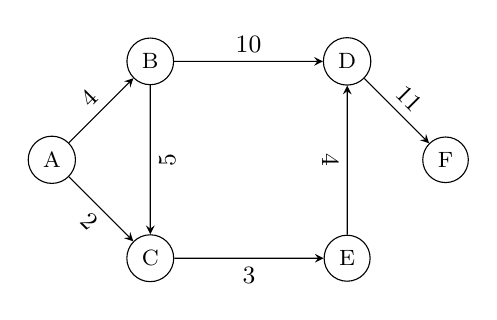
\begin{tikzpicture}[scale=1.25]   
          \small
          \node[node] at (0,0) (A) {A};
          \node[node] at (1,1) (B) {B};
          \node[node] at (1,-1) (C) {C};
          \node[node] at (3,1) (D) {D};
          \node[node] at (3,-1) (E) {E};
          \node[node] at (4,0) (F) {F};

          \draw[arrow] (A) -- (C) node[midway,below, sloped]{2};
          \draw[arrow] (A) -- (B) node[midway,above, sloped]{4};
          \draw[arrow] (B) -- (D) node[midway,above, sloped]{10};
          \draw[arrow] (C) -- (E) node[midway,below, sloped]{3};
          \draw[arrow] (D) -- (F) node[midway,above, sloped]{11};
          \draw[arrow] (B) -- (C) node[midway,below, sloped]{5};
          \draw[arrow] (E) -- (D) node[midway,below, sloped]{4};
        \end{tikzpicture}%
        \caption{\text{\hspace{-0.5cm}}} \label{fig1:a}  
      \end{subfigure}
    \hspace{1cm}
    \begin{subfigure}[t]{0.4\textwidth}
        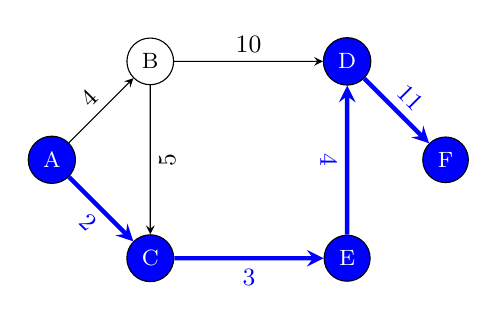
\begin{tikzpicture}[scale=1.25]   
        \small
        \node[node, fill= blue, text=white] at (0,0) (A) {A};
        \node[node] at (1,1) (B) {B};
        \node[node, fill= blue, text=white] at (1,-1) (C) {C};
        \node[node, fill= blue, text=white] at (3,1) (D) {D};
        \node[node, fill= blue, text=white] at (3,-1) (E) {E};
        \node[node, fill= blue, text=white] at (4,0) (F) {F};

        \draw[arrow, blue, ultra thick] (A) -- (C) node[midway,below, sloped]{2};
        \draw[arrow] (A) -- (B) node[midway,above, sloped]{4};
        \draw[arrow] (B) -- (D) node[midway,above, sloped]{10};
        \draw[arrow, blue, ultra thick] (C) -- (E) node[midway,below, sloped]{3};
        \draw[arrow, blue, ultra thick] (D) -- (F) node[midway,above, sloped]{11};
        \draw[arrow] (B) -- (C) node[midway,below, sloped]{5};
        \draw[arrow, blue, ultra thick] (E) -- (D) node[midway,below, sloped]{4};
    \end{tikzpicture}
    \caption{\text{\hspace{-0.5cm}}} \label{fig1:b}   
    \end{subfigure}
    \caption{Illustrates the concept of a shortest path given a source and a destination. \textbf{(a)} shows the original directed graph. \textbf{(b)} identifies the shortest-path (\emph{edges and nodes marked in \textcolor{blue}{blue}}) for $A \xrightarrow{p} F$.\cite{wikipediaImg}}
\end{figure}

\noindent
Having established the shortest path problem as a whole, let us now reveal a slight obfuscation with respect to the scope of the project. Indeed, the project focuses upon the Shortest Path Problem but what was omitted earlier was the intent to focus solely upon the \textbf{Single-Source Shortest Path}
variant. The decision of dealing prime focus to this particular variant originates from the fact the solution to this specific problem in itself solves many other problems in addition to solving the other variants of the Shortest Path problem \cite{cormenBk,sedgewickBk}:

\begin{enumerate}
    \item Single-destination
    \item Single-pair
    \item All-pairs
\end{enumerate}

\noindent
For a graph, $G = (V, E)$, the \textbf{Single-Source Shortest Path} (SSSP) problem consists of finding the shortest paths between a given \textbf{\emph{source}} vertex $s \in V$ to each vertex $v \in V$ \cite{cormenBk,chaupis-et.al:2017}. \textbf{Figures} \ref{fig2:a} and \ref{fig2:b} illustrates this concept.

\begin{figure}[H]  
    \centering 
      \begin{subfigure}[t]{0.4\textwidth}
        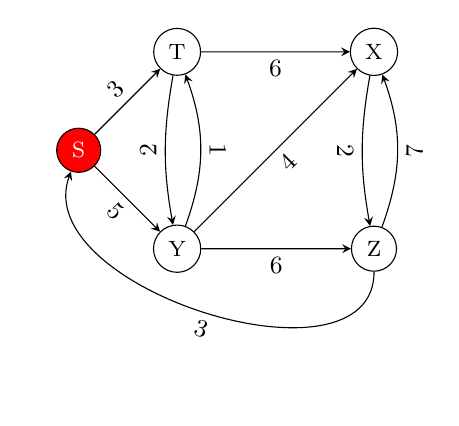
\begin{tikzpicture}[scale=1.25]   
          \small
          \node[node, fill=red, text=white] at (0,0) (S) {S};
          \node[node] at (1,1) (T) {T};
          \node[node] at (1,-1) (Y) {Y};
          \node[node] at (3,1) (X) {X};
          \node[node] at (3,-1) (Z) {Z};

          \draw[arrow] (S) -- (T) node[midway,above, sloped]{3};
          \draw[arrow] (S) -- (Y) node[midway,below, sloped]{5};
          \draw[arrow] (Y) -- (Z) node[midway,below, sloped]{6};
          \draw[arrow] (T) -- (X) node[midway,below, sloped]{6};
          \draw[arrow] (Y) -- (X) node[midway,below, sloped]{4};
          \draw[arrow] (T) to [out=260, in=100] node[midway, above, sloped]{2} (Y);
          \draw[arrow] (Y) to [out=70, in=290] node[midway,above, sloped]{1} (T);
          \draw[arrow] (X) to [out=260, in=100] node[midway, below, sloped]{2} (Z);
          \draw[arrow] (Z) to [out=70, in=290] node[midway,below, sloped]{7} (X);
          \draw[arrow] (Z) to [out=270, in=250] node[midway, below, sloped]{3} (S);
        \end{tikzpicture}%
        \caption{\text{\hspace{-0.5cm}}} \label{fig2:a}  
      \end{subfigure}
    \hspace{1cm}
    \begin{subfigure}[t]{0.4\textwidth}
        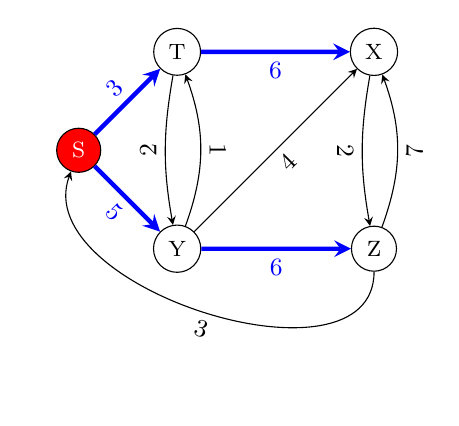
\begin{tikzpicture}[scale=1.25]   
        \small
        \node[node, fill=red, text=white] at (0,0) (S) {S};
        \node[node] at (1,1) (T) {T};
        \node[node] at (1,-1) (Y) {Y};
        \node[node] at (3,1) (X) {X};
        \node[node] at (3,-1) (Z) {Z};

        \draw[arrow, blue, ultra thick] (S) -- (T) node[midway,above, sloped]{3};
        \draw[arrow, blue, ultra thick] (S) -- (Y) node[midway,below, sloped]{5};
        \draw[arrow, blue, ultra thick] (Y) -- (Z) node[midway,below, sloped]{6};
        \draw[arrow, blue, ultra thick] (T) -- (X) node[midway,below, sloped]{6};
        \draw[arrow] (Y) -- (X) node[midway,below, sloped]{4};
        \draw[arrow] (T) to [out=260, in=100] node[midway, above, sloped]{2} (Y);
        \draw[arrow] (Y) to [out=70, in=290] node[midway,above, sloped]{1} (T);
        \draw[arrow] (X) to [out=260, in=100] node[midway, below, sloped]{2} (Z);
        \draw[arrow] (Z) to [out=70, in=290] node[midway,below, sloped]{7} (X);
        \draw[arrow] (Z) to [out=270, in=250] node[midway, below, sloped]{3} (S);
    \end{tikzpicture}
    \caption{\text{\hspace{-0.5cm}}} \label{fig2:b}   
    \end{subfigure}
    \caption{Given a \textbf{source} vertex \(S\), \textbf{(a)} shows the original weighted directed graph with the source vertex marked in \textcolor{red}{red}. \textbf{(b)} shows the same graph from (a) but with the shortest path from the source to every other vertex marked in \textcolor{blue}{blue} - \textbf{Note}: these marked shortest paths are \emph{not unique} (for $S \xrightarrow{p} X$, we have the same minimally costing path if we took the edges \((S, Y), (Y, X)\) as well).\cite{cormenBk}}
\end{figure}

\chapter{Algorithms \& Design Techniques}
\label{chap:3}
The project will be focusing on two algorithmic paradigms/design techniques to solve the problem in question. We will considering a \textbf{greedy approach} (i.e., \textit{Dijkstra's algorithm}) and a \textbf{dynamic-programming approach} (i.e., \textit{Bellman-Ford algorithm}).
In later chapters, we shall compare both these approaches for the given problem both, theoretically (i.e., \emph{asymptotically}) and empirically.

\section{Bellman-Ford}
The \emph{\textbf{Bellman-Ford}} algorithm solves the single-source shortest-paths problem in the general case in which edge weights \emph{may be negative} \cite{cormenBk}. Given a \textbf{weighted}, \textbf{directed} graph \(G = (V, E)\) with source, \(s\) and weight function $w: E \rightarrow \mathbb{R}$,
we want to compute the shortest path distance \(\delta(s, v)\) from source $s$ for all $v \in V$ \cite{stand:bford:11,cormenBk}. More specifically, the Bellman-Ford algorithm:
\begin{itemize}
    \item Detects a negative cycle \emph{if it exists and is reachable} from \(s\), or
    \item Computes the shortest path distances $\delta(s, v)$ for all $v \in V$.
\end{itemize}
In short, if a negative weight cycle is found, then algorithm proceeds to indicate that a \emph{solution does not exist} otherwise, it produces the shortest paths and their weights \cite{cormenBk,stand:bford:11}.

Having introduced the algorithm, let us now proceed with the Dynamic Programming underpinnings. How can we use Dynamic Programming to find the shortest path from a source \(s\) to all other vertices?
First of all, lets just compute the \emph{lengths} of the shortest paths first, and afterwards we can use these lengths to easily reconstruct the paths themselves \cite{toyota:2019}. Next, to use Dynamic Programming, we need to define subproblems.
These subproblems in queston, will be finding the shortest path from source \(s\) to every other vertex that uses \(k\) or fewer edges, \emph{if such a path exists} \cite{toyota:2019}. More specifically, the algorithm proceeds as follows:
\begin{enumerate}
    \item For each vertex, \(v\), find the length of the shortest path to this vertex from the source \(s\) that uses at most 1 edge, or simply specify \(\infty\) if there is no such path.
    
    \textbf{This is trivial}: if $s = v$, we get 0; if $(s, v) \in E$ then we simply specify $w(s, v)$; else we specify \(\infty\) \cite{cormenBk,toyota:2019}.
    \item Now, suppose $\forall v$ we have solved for length of the shortest path from \(s\) that uses \(k - 1\) or fewer edges. How can we use this to solve for the shortest path that uses \(k\) or fewer edges?
    
    \textbf{Answer}: the shortest path from \(s\) to \(v\) that uses \(k\) or fewer edges wil first go to some neighbor, \(u\) of \(v\), and then take the shortest path from \(u\) to \(v\) that uses \(k - 1\) or fewer edges, 
    \emph{\textbf{which we have already solved for}}. Thus, we simply take the minimum over all neighbors \(u\) of \(v\) \cite{toyota:2019,stand:bford:12}. We rely on the following recurrence relation between the intermediate solutions:
    \begin{equation}
        v.d_{k} = \min_{u \in V}\{u.d_{k-1} + w(u, v)\},
    \end{equation}
    where $v.d_{k}$ is the length of the shortest path from source \(s\) to vertex \(v\) using at most \(k\) edges, and \(w(u, v)\) is the weight of the edge \((u, v)\) \cite{toyota:2019,stand:bford:12}.  
    \item How far do we need to go?
    
    \textbf{Answer}: at most \(k = |V| - 1\) edges. Why? Because more than that will create a cycle, and we can then just cut out the cycle to get a shorter path (\emph{remember there are no negative-weight cycles}) \cite{toyota:2019}.
\end{enumerate}

\subsection{Algorithm}
With the aforementioned discussion, the algorithm follows quite simply. 

\begin{center}
    \colorbox[gray]{0.95}{
      \begin{minipage}{\textwidth}
        \SetAlgoLined
        % \setstretch{1.20}
        \begin{algorithm}[H]
          \DontPrintSemicolon
            \small
            $v.d \gets \infty, \forall v \in V$ // set initial distance estimates\;
            // maintain paths: set $v.\pi \gets NIL$ for all \(v\), \(v.\pi\) denotes the predecessor of \(v\)\;
            $s.d \gets 0$ // set distance to source trivially as 0\;
            \For {$i \gets 1$ \textbf{\emph{to}} \(|G.V| - 1\)}
            {
                \For {\textbf{\emph{each edge}} $(u, v) \in G.E$}
                {
                    // relaxation of edges\;
                    $v.d \gets min\{ v.d, u.d + w(u, v) \}$ // update the distance estimate for \(v\)\;
                    // maintain paths: if $v.d$ changes, then $v.\pi \gets u$\; 
                }
            }
            // negative cycle step\;
            \For {\textbf{\emph{each edge}} $(u, v) \in G.E$}
            {
                \If{$v.d > u.d + w(u, v)$}
                {
                    \Return{\emph{FALSE}} // negative cycle detected\;
                }
            }

            \Return{$v.d \; \forall v \in V$}\;

        \caption{\small\color{purple} BELLMAN-FORD \cite{stand:bford:11,cormenBk}}
        \label{alg:BFord}
        \end{algorithm}
      \end{minipage}}
\end{center}

\subsection{An Example}
\textbf{Figures} (\ref{fig3:a}) - (\ref{fig3:e}) showcase the execution of \textbf{Algorithm} \ref{alg:BFord} on a graph with 5 vertices.

\begin{figure}[H]  
    \centering 
      \begin{subfigure}[t]{0.3\textwidth}
        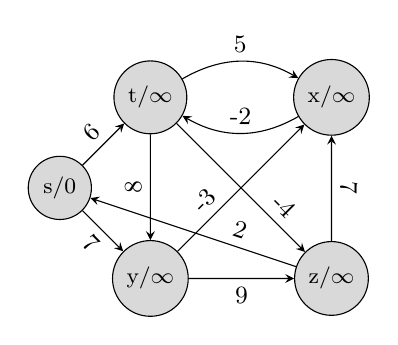
\begin{tikzpicture}[scale=1.15]   
          \small
          \node[node, fill=gray!30] at (0,0) (s) {s/0};
          \node[node, fill=gray!30] at (3,1) (x) {x/\(\infty\)};
          \node[node, fill=gray!30] at (1,1) (t) {t/\(\infty\)};
          \node[node, fill=gray!30] at (1,-1) (y) {y/\(\infty\)};
          \node[node, fill=gray!30] at (3,-1) (z) {z/\(\infty\)};

          \draw[arrow] (s) -- (t) node[midway,above, sloped]{6};
          \draw[arrow] (s) -- (y) node[midway,below, sloped]{7};
          \draw[arrow] (t) -- (y) node[midway,above, sloped]{8};
          \draw[arrow] (y) -- (x) node[midway,above, sloped]{\hspace{-1cm} -3};
          \draw[arrow] (y) -- (z) node[midway,below, sloped]{9};
          \draw[arrow] (z) -- (x) node[midway,above, sloped]{7};
          \draw[arrow] (z) -- (s) node[midway,above, sloped]{\hspace{1cm} 2};
          \draw[arrow] (t) -- (z) node[midway,above, sloped]{\hspace{1cm} -4};
          \draw[arrow] (x) to [out=210, in=-30] node[midway,above, sloped]{-2} (t);
          \draw[arrow] (t) to [out=30, in=150] node[midway,above, sloped]{5} (x);
        \end{tikzpicture}%
        \caption{\text{\hspace{-1cm}}} \label{fig3:a}  
      \end{subfigure}
    \hspace{0.35cm}
    \begin{subfigure}[t]{0.3\textwidth}
        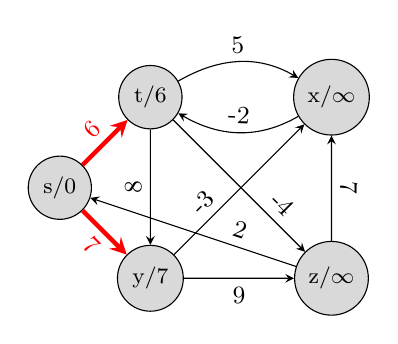
\begin{tikzpicture}[scale=1.15]   
        \small
        \node[node, fill=gray!30] at (0,0) (s) {s/0};
        \node[node, fill=gray!30] at (3,1) (x) {x/\(\infty\)};
        \node[node, fill=gray!30] at (1,1) (t) {t/6};
        \node[node, fill=gray!30] at (1,-1) (y) {y/7};
        \node[node, fill=gray!30] at (3,-1) (z) {z/\(\infty\)};

        \draw[red, arrow, ultra thick] (s) -- (t) node[midway,above, sloped]{6};
        \draw[red, arrow, ultra thick] (s) -- (y) node[midway,below, sloped]{7};
        \draw[arrow] (t) -- (y) node[midway,above, sloped]{8};
        \draw[arrow] (y) -- (x) node[midway,above, sloped]{\hspace{-1cm} -3};
        \draw[arrow] (y) -- (z) node[midway,below, sloped]{9};
        \draw[arrow] (z) -- (x) node[midway,above, sloped]{7};
        \draw[arrow] (z) -- (s) node[midway,above, sloped]{\hspace{1cm} 2};
        \draw[arrow] (t) -- (z) node[midway,above, sloped]{\hspace{1cm} -4};
        \draw[arrow] (x) to [out=210, in=-30] node[midway,above, sloped]{-2} (t);
        \draw[arrow] (t) to [out=30, in=150] node[midway,above, sloped]{5} (x);

    \end{tikzpicture}
    \caption{\text{\hspace{-1cm}}} \label{fig3:b}  
    \end{subfigure}
    \hspace{0.35cm}
    \begin{subfigure}[t]{0.3\textwidth}
        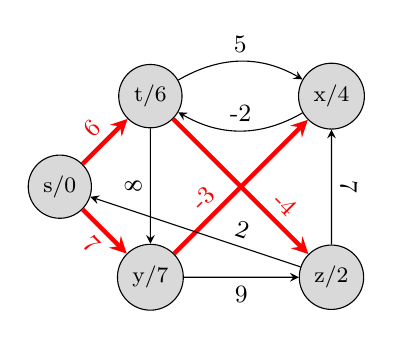
\begin{tikzpicture}[scale=1.15]   
        \small
        \node[node, fill=gray!30] at (0,0) (s) {s/0};
        \node[node, fill=gray!30] at (3,1) (x) {x/4};
        \node[node, fill=gray!30] at (1,1) (t) {t/6};
        \node[node, fill=gray!30] at (1,-1) (y) {y/7};
        \node[node, fill=gray!30] at (3,-1) (z) {z/2};

        \draw[red, arrow, ultra thick] (s) -- (t) node[midway,above, sloped]{6};
        \draw[red, arrow, ultra thick] (s) -- (y) node[midway,below, sloped]{7};
        \draw[arrow] (t) -- (y) node[midway,above, sloped]{8};
        \draw[red, arrow, ultra thick] (y) -- (x) node[midway,above, sloped]{\hspace{-1cm} -3};
        \draw[arrow] (y) -- (z) node[midway,below, sloped]{9};
        \draw[arrow] (z) -- (x) node[midway,above, sloped]{7};
        \draw[arrow] (z) -- (s) node[midway,above, sloped]{\hspace{1cm} 2};
        \draw[red, arrow, ultra thick] (t) -- (z) node[midway,above, sloped]{\hspace{1cm} -4};
        \draw[arrow] (x) to [out=210, in=-30] node[midway,above, sloped]{-2} (t);
        \draw[arrow] (t) to [out=30, in=150] node[midway,above, sloped]{5} (x);

      \end{tikzpicture}%
      \caption{\text{\hspace{-1cm}}} \label{fig3:c}  
    \end{subfigure}
    \begin{subfigure}[t]{0.3\textwidth}
        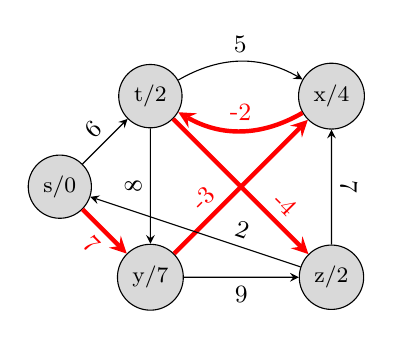
\begin{tikzpicture}[scale=1.15]   
        \small
        \node[node, fill=gray!30] at (0,0) (s) {s/0};
        \node[node, fill=gray!30] at (3,1) (x) {x/4};
        \node[node, fill=gray!30] at (1,1) (t) {t/2};
        \node[node, fill=gray!30] at (1,-1) (y) {y/7};
        \node[node, fill=gray!30] at (3,-1) (z) {z/2};

        \draw[arrow] (s) -- (t) node[midway,above, sloped]{6};
        \draw[red, arrow, ultra thick] (s) -- (y) node[midway,below, sloped]{7};
        \draw[arrow] (t) -- (y) node[midway,above, sloped]{8};
        \draw[red, arrow, ultra thick] (y) -- (x) node[midway,above, sloped]{\hspace{-1cm} -3};
        \draw[arrow] (y) -- (z) node[midway,below, sloped]{9};
        \draw[arrow] (z) -- (x) node[midway,above, sloped]{7};
        \draw[arrow] (z) -- (s) node[midway,above, sloped]{\hspace{1cm} 2};
        \draw[red, arrow, ultra thick] (t) -- (z) node[midway,above, sloped]{\hspace{1cm} -4};
        \draw[red, arrow, ultra thick] (x) to [out=210, in=-30] node[midway,above, sloped]{-2} (t);
        \draw[arrow] (t) to [out=30, in=150] node[midway,above, sloped]{5} (x);
        \end{tikzpicture}%
        \caption{\text{\hspace{-1cm}}} \label{fig3:d}  
      \end{subfigure}
    \hspace{0.35cm}
    \begin{subfigure}[t]{0.3\textwidth}
        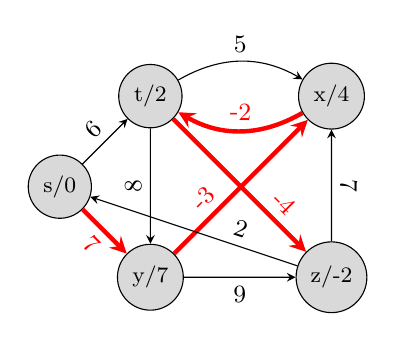
\begin{tikzpicture}[scale=1.15]   
        \small
        \node[node, fill=gray!30] at (0,0) (s) {s/0};
        \node[node, fill=gray!30] at (3,1) (x) {x/4};
        \node[node, fill=gray!30] at (1,1) (t) {t/2};
        \node[node, fill=gray!30] at (1,-1) (y) {y/7};
        \node[node, fill=gray!30] at (3,-1) (z) {z/-2};

        \draw[arrow] (s) -- (t) node[midway,above, sloped]{6};
        \draw[red, arrow, ultra thick] (s) -- (y) node[midway,below, sloped]{7};
        \draw[arrow] (t) -- (y) node[midway,above, sloped]{8};
        \draw[red, arrow, ultra thick] (y) -- (x) node[midway,above, sloped]{\hspace{-1cm} -3};
        \draw[arrow] (y) -- (z) node[midway,below, sloped]{9};
        \draw[arrow] (z) -- (x) node[midway,above, sloped]{7};
        \draw[arrow] (z) -- (s) node[midway,above, sloped]{\hspace{1cm} 2};
        \draw[red, arrow, ultra thick] (t) -- (z) node[midway,above, sloped]{\hspace{1cm} -4};
        \draw[red, arrow, ultra thick] (x) to [out=210, in=-30] node[midway,above, sloped]{-2} (t);
        \draw[arrow] (t) to [out=30, in=150] node[midway,above, sloped]{5} (x);

    \end{tikzpicture}
    \caption{\text{\hspace{-1cm}}} \label{fig3:e}  
    \end{subfigure}
    \caption{The execution of the Bellman-Ford algorithm. The source vertex is \(s\). The \(d\) values appear within the vertices, and the \textcolor{red}{red edges}
    indicate predecessor values: if \((u, v)\) is shaded, the \(v.\pi = u\). In this particular example, each pass relaxes the edges in the order
    $(t, x), (t, y), (t, z), (x, t), (y, x), (y, z) (z, x), (z, s), (s, t)  (s, y)$. \textbf{(a)} The situation just before the
    first pass over the edges. \textbf{(b) - (e)} The situation after each successive pass over the edges. The \(d\) and $\pi$ values in part \textbf{(e)} are the final values.
    The Bellman-Ford algorithm returns \texttt{TRUE} in this example. \cite{cormenBk}}
\end{figure}

\subsection{A Note on Negative Weight Cycles}
Before we conclude our discussion on Bellman-Ford, let us first elaborate upon, the algorithm's working with respect to negative weight cycles reachable from the source, \(s\).

\begin{claim}
\emph{If there is a negative cycle reachable from s, then the Bellman-Ford algorithm detects and reports
``FALSE”}.
\end{claim}

\begin{claimproof}
For the sake of contradiction, suppose there exists a negative cycle, \(C\) reachable fromt the source, \(s\) and the Bellman-Ford algorithm does not report \texttt{FALSE}.
Assume \(C\) contains nodes \(v_{1}, v_{2}, \ldots, v_{k}\) with edges \((v_{i}, v_{i + 1})\) for \(i = 1, \ldots, k\) such that $\sum_{i=1}^{k} w(v_{i}, v_{i + 1}) < 0$, where
\(v_{k + 1} = v_{1}\) \cite{cormenBk,stand:bford:11}. \textbf{Figure} \ref{fig4:negweight} presents this scenario.

\begin{figure}[H]
    \centering
    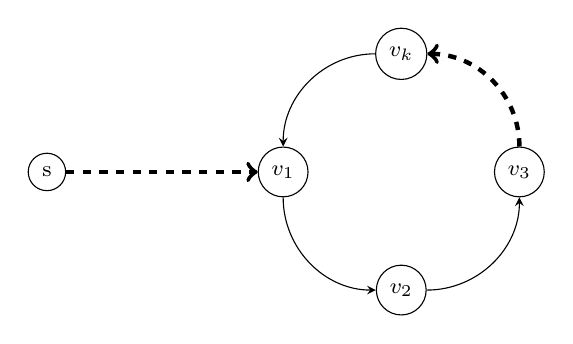
\begin{tikzpicture}[scale=1.5,baseline=(current bounding box.center)]
        \small
        \node[node] at (-2, 0) (s) {s};
        \node[node] at (0, 0) (a) {$v_{1}$};
        \node[node] at (1,-1) (b) {$v_{2}$};
        \node[node] at (2, 0) (c) {$v_{3}$};
        \node[node] at (1, 1) (d) {$v_{k}$};
  
        \draw[dashed, ->, ultra thick] (s) -- (a);
        \draw[arrow] (a) to [out=270, in=180]  (b);
        \draw[arrow] (b) to [out=0, in=270]  (c);
        \draw[dashed, ->, ultra thick] (c) to [out=90, in=0]  (d);
        \draw[arrow] (d) to [out=180, in=90]  (a);
    \end{tikzpicture}
    \caption{A negative weight cycle reachable from the source, \(s\).}
    \label{fig4:negweight}
\end{figure}

Since \(C\) is reachable from \(s\), there is a path from \(s\) to \(v_{1}\) and to all nodes on \(C\). In particular, there exist simple paths, i.e., paths without cycles, of at most \(|V| - 1\)
edges to the nodes of \(C\). In the first for-loop, the edges on each such simple path get relaxed in order and consequently, \(v_{i}.d\) will be some finite number less than \(\infty\) for \(i = 1, \ldots, k\).
Since the Bellman-Ford algorithm does not report \texttt{FALSE} in the second for loop (\emph{lines 12-16 of Algorithm} \ref{alg:BFord}), it must be that
$v_{i+1}.d \leq v_{i}.d + w(v_{i}, v_{i+1})$ for $i = 1, \ldots, k$ \cite{cormenBk,stand:bford:11}. Adding the inequalities, we obtain:
\begin{equation}
    \sum_{i=1}^{k} v_{i+1}.d \leq  \sum_{i=1}^{k} v_{i}.d + \sum_{i=1}^{k} w(v_{i}, v_{i+1}) .  
\end{equation}
As we are summing over the cycle, \(C\), the terms $\sum_{i=1}^{k} v_{i+1}.d$ and $\sum_{i=1}^{k} v_{i}.d$ are equal and can be cancelled. It follows that $0 \leq \sum_{i=1}^{k} w(v_{i}, v_{i+1})$. This contradicts that \(C\)
is a negative cycle \cite{cormenBk,stand:bford:11}.
\end{claimproof}

\section{Dijkstra's}
\label{sec:3.2}
\textbf{Dijkstra's} algorithm solves the single-source shortest-paths problem on a \textbf{weighted}, \textbf{directed} graph \(G = (V, E)\) for the case in which all edge weights are non-negative \cite{cormenBk}. An edge \((u, v) \in E\) has weight \(w(u, v)\).
The key idea behind Dijkstra's algorithm is to maintain an estimate of the current shortest path ending at \(v\) for \(v \in V\) over the iterations \cite{stand:bford:12}. More specifically, the algorithm computes an estimate of the distance of \(v\) from the source \(s\), \(v.d\), such that:
\begin{enumerate}
    \item At any point in time, \(v.d \geq \delta(s, v)\), and
    \item When \(v\) is finished, $v.d = \delta(s, v)$.
\end{enumerate}
To be precise, the algorithm maintains a set, \(S\) of vertices whose final shortest path weights from the source \(s\) have been computed. Thus, the algorithm repeatedly selects a vertex \(u \in V - S\) (i.e., \emph{from \(Q\), a minimum priority queue of vertices keyed on the d-values})
with the minimum shortest path estimate, adds \(u\) to the set \(S\), and in turn, relaxes all edges leaving \(u\) \cite{cormenBk,stand:bford:12}. Since Dijkstra's algorithm always chooses the ``lightest'' or ``closest'' vertex in \(V-S\) to add to set \(S\) thus, the algorithm utilizes a \emph{\textbf{greedy}} strategy.

\subsection{Algorithm}
\begin{center}
    \colorbox[gray]{0.95}{
      \begin{minipage}{0.7\textwidth}
        \SetAlgoLined
        % \setstretch{1.20}
        \begin{algorithm}[H]
          \DontPrintSemicolon
          INITIALIZE-SINGLE-SOURCE(\(G, s\))\;
          $S = \emptyset$\;
          $Q = G.V$\;
          \While{$Q \not = \emptyset$}
          {
            $u \gets$ \emph{EXTRACT-MIN}(\(Q\))\;
            $S \gets S \cup \{u\}$\;
            \For{\textbf{\emph{each vertex}} $v \in G.Adj[u]$}
            {
                \emph{RELAX}(\(u, v, w\))\;
            }
          }
          \caption{\small\color{purple} DIJKSTRA \color{black}(\(G, w, s\)) \cite{cormenBk}}
          \label{alg:dijkstra}
        \end{algorithm}
      \end{minipage}}
\end{center}

Line 1 of the algorithm performs intialization in a manner no different than that of Bellman-Ford (\emph{lines 1-3 of Algorithm \ref{alg:BFord}}).
Line 2 initializes the set \(S\) to the empty set and line 3 proceeds to place all vertices $\in V$ in the priority queue. The remainder of the algorithm, 
\emph{lines 4-10}, proceed as described beforehand in \textbf{Section} \ref{sec:3.2}. 

\subsection{An Example}
\textbf{Figures} \ref{fig5:a} - \ref{fig5:f} showcase the execution of Algorithm \ref{alg:dijkstra} on a graph with 5 vertices.
\begin{figure}[H]  
    \centering 
      \begin{subfigure}[t]{0.3\textwidth}
        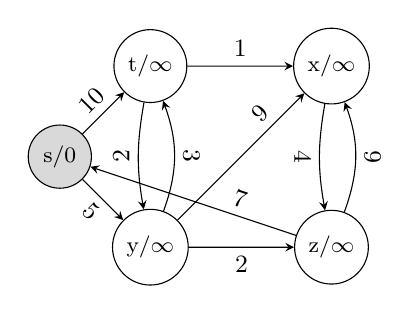
\begin{tikzpicture}[scale=1.15]   
          \small
          \node[node, fill=gray!30] at (0,0) (s) {s/0};
          \node[node] at (3,1) (x) {x/\(\infty\)};
          \node[node] at (1,1) (t) {t/\(\infty\)};
          \node[node] at (1,-1) (y) {y/\(\infty\)};
          \node[node] at (3,-1) (z) {z/\(\infty\)};

          \draw[arrow] (s) -- (t) node[midway,above, sloped]{10};
          \draw[arrow] (s) -- (y) node[midway,below, sloped]{5};
          \draw[arrow] (t) to [out=260, in=100] node[midway, above, sloped]{2} (y);
          \draw[arrow] (y) to [out=70, in=290] node[midway,above, sloped]{3} (t);
          \draw[arrow] (t) -- (x) node[midway,above, sloped]{1};
          \draw[arrow] (x) to [out=260, in=100] node[midway, below, sloped]{4} (z);
          \draw[arrow] (z) to [out=70, in=290] node[midway,below, sloped]{6} (x);
          \draw[arrow] (y) -- (z) node[midway,below, sloped]{2};
          \draw[arrow] (z) -- (s) node[midway,above, sloped]{\hspace{1cm} 7};
          \draw[arrow] (y) -- (x) node[midway,above, sloped]{\hspace{1cm} 9};
        \end{tikzpicture}%
        \caption{\text{\hspace{-1cm}}} \label{fig5:a}  
      \end{subfigure}
    \hspace{0.35cm}
    \begin{subfigure}[t]{0.3\textwidth}
        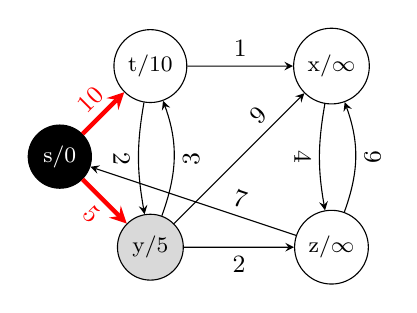
\begin{tikzpicture}[scale=1.15]   
        \small
        \node[node, fill=black, text=white] at (0,0) (s) {s/0};
        \node[node] at (1,1) (t) {t/10};
        \node[node, fill=gray!30] at (1,-1) (y) {y/5};
        \node[node] at (3,1) (x) {x/\(\infty\)};
        \node[node] at (3,-1) (z) {z/\(\infty\)};

        \draw[arrow, red, ultra thick] (s) -- (t) node[midway,above, sloped]{10};
        \draw[arrow, red, ultra thick] (s) -- (y) node[midway,below, sloped]{5};
        \draw[arrow] (t) to [out=260, in=100] node[midway, below, sloped]{2} (y);
        \draw[arrow] (y) to [out=70, in=290] node[midway,below, sloped]{3} (t);
        \draw[arrow] (t) -- (x) node[midway,above, sloped]{1};
        \draw[arrow] (x) to [out=260, in=100] node[midway, below, sloped]{4} (z);
        \draw[arrow] (z) to [out=70, in=290] node[midway,below, sloped]{6} (x);
        \draw[arrow] (y) -- (z) node[midway,below, sloped]{2};
        \draw[arrow] (z) -- (s) node[midway,above, sloped]{\hspace{1cm} 7};
        \draw[arrow] (y) -- (x) node[midway,above, sloped]{\hspace{1cm} 9};
    \end{tikzpicture}
    \caption{\text{\hspace{-1cm}}} \label{fig5:b}  
    \end{subfigure}
    \hspace{0.35cm}
    \begin{subfigure}[t]{0.3\textwidth}
        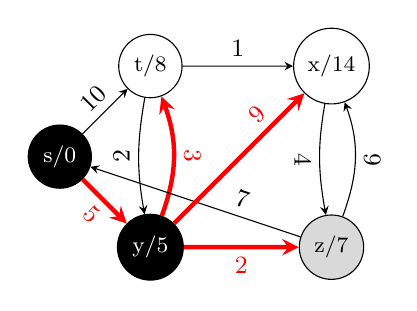
\begin{tikzpicture}[scale=1.15]   
        \small
        \node[node, fill=black, text=white] at (0,0) (s) {s/0};
        \node[node] at (1,1) (t) {t/8};
        \node[node, fill=black, text=white] at (1,-1) (y) {y/5};
        \node[node] at (3,1) (x) {x/14};
        \node[node, fill=gray!30] at (3,-1) (z) {z/7};

        \draw[arrow] (s) -- (t) node[midway,above, sloped]{10};
        \draw[arrow, red, ultra thick] (s) -- (y) node[midway,below, sloped]{5};
        \draw[arrow] (t) to [out=260, in=100] node[midway, above, sloped]{2} (y);
        \draw[arrow, red, ultra thick] (y) to [out=70, in=290] node[midway,above, sloped]{3} (t);
        \draw[arrow] (t) -- (x) node[midway,above, sloped]{1};
        \draw[arrow] (x) to [out=260, in=100] node[midway, below, sloped]{4} (z);
        \draw[arrow] (z) to [out=70, in=290] node[midway,below, sloped]{6} (x);
        \draw[arrow, red, ultra thick] (y) -- (z) node[midway,below, sloped]{2};
        \draw[arrow] (z) -- (s) node[midway,above, sloped]{\hspace{1cm} 7};
        \draw[arrow, red, ultra thick] (y) -- (x) node[midway,above, sloped]{\hspace{1cm} 9};

      \end{tikzpicture}%
      \caption{\text{\hspace{-1cm}}} \label{fig5:c}  
    \end{subfigure}
    \begin{subfigure}[t]{0.3\textwidth}
        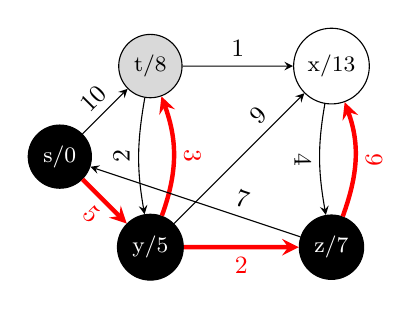
\begin{tikzpicture}[scale=1.15]   
        \small
        \node[node, fill=black, text=white] at (0,0) (s) {s/0};
        \node[node, fill=gray!30] at (1,1) (t) {t/8};
        \node[node, fill=black, text=white] at (1,-1) (y) {y/5};
        \node[node] at (3,1) (x) {x/13};
        \node[node, fill=black, text=white] at (3,-1) (z) {z/7};

        \draw[arrow] (s) -- (t) node[midway,above, sloped]{10};
        \draw[arrow, red, ultra thick] (s) -- (y) node[midway,below, sloped]{5};
        \draw[arrow] (t) to [out=260, in=100] node[midway, above, sloped]{2} (y);
        \draw[arrow, red, ultra thick] (y) to [out=70, in=290] node[midway,above, sloped]{3} (t);
        \draw[arrow] (t) -- (x) node[midway,above, sloped]{1};
        \draw[arrow] (x) to [out=260, in=100] node[midway, below, sloped]{4} (z);
        \draw[arrow, red, ultra thick] (z) to [out=70, in=290] node[midway,below, sloped]{6} (x);
        \draw[arrow, red, ultra thick] (y) -- (z) node[midway,below, sloped]{2};
        \draw[arrow] (z) -- (s) node[midway,above, sloped]{\hspace{1cm} 7};
        \draw[arrow] (y) -- (x) node[midway,above, sloped]{\hspace{1cm} 9};
        \end{tikzpicture}%
        \caption{\text{\hspace{-1cm}}} \label{fig5:d}  
      \end{subfigure}
    \hspace{0.35cm}
    \begin{subfigure}[t]{0.3\textwidth}
        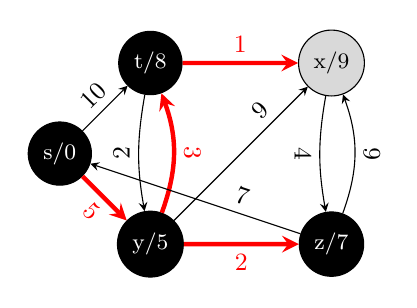
\begin{tikzpicture}[scale=1.15]   
        \small
        \node[node, fill=black, text=white] at (0,0) (s) {s/0};
        \node[node, fill=black, text=white] at (1,1) (t) {t/8};
        \node[node, fill=black, text=white] at (1,-1) (y) {y/5};
        \node[node, fill=gray!30] at (3,1) (x) {x/9};
        \node[node, fill=black, text=white] at (3,-1) (z) {z/7};

        \draw[arrow] (s) -- (t) node[midway,above, sloped]{10};
        \draw[arrow, red, ultra thick] (s) -- (y) node[midway,below, sloped]{5};
        \draw[arrow] (t) to [out=260, in=100] node[midway, above, sloped]{2} (y);
        \draw[arrow, red, ultra thick] (y) to [out=70, in=290] node[midway,above, sloped]{3} (t);
        \draw[arrow, red, ultra thick] (t) -- (x) node[midway,above, sloped]{1};
        \draw[arrow] (x) to [out=260, in=100] node[midway, below, sloped]{4} (z);
        \draw[arrow] (z) to [out=70, in=290] node[midway,below, sloped]{6} (x);
        \draw[arrow, red, ultra thick] (y) -- (z) node[midway,below, sloped]{2};
        \draw[arrow] (z) -- (s) node[midway,above, sloped]{\hspace{1cm} 7};
        \draw[arrow] (y) -- (x) node[midway,above, sloped]{\hspace{1cm} 9};

    \end{tikzpicture}
    \caption{\text{\hspace{-1cm}}} \label{fig5:e}  
    \end{subfigure}
    \hspace{0.35cm}
    \begin{subfigure}[t]{0.3\textwidth}
        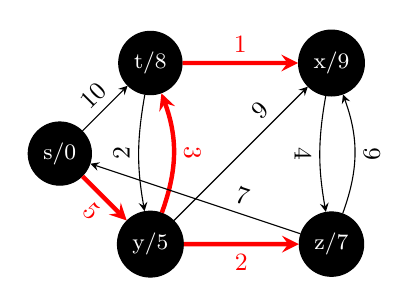
\begin{tikzpicture}[scale=1.15]   
        \small
        \node[node, fill=black, text=white] at (0,0) (s) {s/0};
        \node[node, fill=black, text=white] at (1,1) (t) {t/8};
        \node[node, fill=black, text=white] at (1,-1) (y) {y/5};
        \node[node, fill=black, text=white] at (3,1) (x) {x/9};
        \node[node, fill=black, text=white] at (3,-1) (z) {z/7};

        \draw[arrow] (s) -- (t) node[midway,above, sloped]{10};
        \draw[arrow, red, ultra thick] (s) -- (y) node[midway,below, sloped]{5};
        \draw[arrow] (t) to [out=260, in=100] node[midway, above, sloped]{2} (y);
        \draw[arrow, red, ultra thick] (y) to [out=70, in=290] node[midway,above, sloped]{3} (t);
        \draw[arrow, red, ultra thick] (t) -- (x) node[midway,above, sloped]{1};
        \draw[arrow] (x) to [out=260, in=100] node[midway, below, sloped]{4} (z);
        \draw[arrow] (z) to [out=70, in=290] node[midway,below, sloped]{6} (x);
        \draw[arrow, red, ultra thick] (y) -- (z) node[midway,below, sloped]{2};
        \draw[arrow] (z) -- (s) node[midway,above, sloped]{\hspace{1cm} 7};
        \draw[arrow] (y) -- (x) node[midway,above, sloped]{\hspace{1cm} 9};

    \end{tikzpicture}
    \caption{\text{\hspace{-1cm}}} \label{fig5:f}  
    \end{subfigure}
    \caption{The execution of Dijkstra's algorithm. The source vertex \(s\) is the leftmost vertex. The shortest-path estimates appear
    within the vertices, and shaded edges indicate predecessor values. Black vertices are in the set \(S\), and white vertices are in the min-priority
    queue, \(Q\) = \(V-S\). \textbf{(a)} The situation just before the first iteration of the while-loop of \emph{lines 4-9 of Algorithm \ref{alg:dijkstra}}
    . The shaded vertex has the minimum \(d\)-value and is extracted from \(Q\) in line 5. \textbf{(b)-(f)} The situation after each successive iteration of the 
    while loop. The shaded vertex in each part is chosen as vertex \(u\) in line 5 of the next iteration. The \(d\) values and predecessors shown in part (f) are the
    final values. \cite{cormenBk}}
\end{figure}

\chapter{Theoretical Time Complexities}
\section{Bellman-Ford}
Keeping Algorithm \ref{alg:BFord} in mind, we know that after initializing the \(d\) and \(\pi\) values in \emph{lines 1-3}, the algorithm in question
makes  \(|V| - 1\) passes over the edges of the graph \cite{cormenBk}. A single pass constitutes a single iteration of the \textbf{for-loop} of \emph{lines 4-10} and consists
of relaxing each edge once. After concluding the \(|V| - 1\) passes, the algorithm proceeds to check for a negative weight cycle and returns the appropriate boolean value \cite{cormenBk}.

Thus, the algorithm in question runs in \(O(VE)\) time \cite{cormenBk,stand:bford:11,toyota:2019}:
\begin{itemize}
  \item Intialization in \emph{line 1-3} takes \(\Theta(1)\) time
  \item The \textbf{for-loop} of \emph{lines 4-10} amounts to \(|V| - 1\) iterations that take \(\Theta(E)\) time. This totals to \(O(VE)\) time.
  \item The check for a negative weight cycle takes \(O(E)\) time.  
\end{itemize}

\section{Dijkstra}
The priority queue, \(Q\) in Algorithm \ref{alg:dijkstra}, is maintained by calling three priority queue operations: \textbf{INSERT} (\emph{implict in line 3}), \textbf{EXTRACT-MIN} (\emph{line 5})
and \textbf{DECREASE-KEY} (\emph{implicit in the} RELAX \emph{fucntion called in line 8}). Both \textbf{INSERT} and \textbf{EXTRACT} \textbf{-MIN} are called once per vertex \cite{cormenBk}. Since each vertex \(u \in V\) is added to the
set, \(S\) once, thus,  each edge in the adjacency list \(Adj[u]\) is examined only once - within the \textbf{for-loop} of \emph{lines 7-9}. Since all adjacency lists total to \(|E|\) edges thus, the aforementioned loop
is called a total of \(|E|\) times thus, \textbf{DECREASE-KEY} is called at most \(|E|\) times overall \cite{cormenBk}.
\textbf{Table} \ref{tab1:dijkstra} presents a summary of this information.
\begin{table}[H]
  \begin{center}
      \begin{tabular}{ |c|c|c| } 
          \hline
          \textbf{Operation} & \textbf{Time} & \textbf{Occurrences in Dijkstra} \\ 
          \hline
          INSERT(\(X\)) (\(n = |X|\)) & \(I_{n}\) & 1\\
          EXTRACT-MIN & $M_{n}$ & $|V|$\\
          DECREASE-KEY & \(D_{n}\) & \(|E|\)\\
          \hline        
      \end{tabular}
  \end{center}
  \caption{Operations on changeable priority queue, \(Q\), assuming it contains \(n\) items. \cite{ocw:2020}}
  \label{tab1:dijkstra}
\end{table}
Thus, from \textbf{Table} \ref{tab1:dijkstra}, the total running time is $O(I_{|V|} + |V| \cdot M_{|V|} + |E| \cdot D_{|V|})$ \cite{ocw:2020}.

Moreover, we have that the time of the algorithm in question, in fact, additionally depends on how we implement the min-priority queue itself \cite{cormenBk,ocw:2020}. 
Granted that the queue can be implemented using a variety of data structures however, within the scope of this particular project, we restrict the 
discussion solely to the appraches tested - i.e., an \textbf{Array}-based and a \textbf{Binary-Heap} implementation. 

With respect to the \textbf{Array}-based implementation, we simply store the \(v.d\) value in the \(v^{th}\) entry of the array. Each INSERT and 
DECREASE-KEY operation takes \(O(1)\) time. EXTRACT-MIN however, takes \(O(V)\) time since we have to search the entire array to find the minimum vertex.
Thus, we get a runtime of $O(V^{2} + E) \implies O(V^{2})$ time \cite{cormenBk,stand:bford:12,ocw:2020}.

Moving onto the Binary-Heap, each EXTRACT-MIN operation takes \(O(\log V)\) and there are \(|V|\) such operations. 
The time to build the heap itself is \(O(V)\). Each DECREASE-KEY operations takes \(O(\log V)\) time and there \(|E|\) such operations. Thus, the total 
running time ends up being $O((V + E) \log V) \implies O(V\log V)$ time \cite{cormenBk,stand:bford:12,ocw:2020}. 

\textbf{Table} \ref{tab2:dijkstra} compares the two different queue implementations together.

\begin{table}[H]
  \begin{center}
    \begin{tabular}{|l|*{5}{c|}}
      \hline
      \multirow{2}{8em}{Queue Implementation} & \multicolumn{3}{|c|}{Queue Operations \(O(\cdot)\)} &  \multirow{2}{8em}{Dijkstra \(O(\cdot)\) \(n = |V| = O(|E|)\)}\\ \cline{2-4}
      & \footnotesize INSERT & \footnotesize EXTRACT-MIN & \footnotesize DECREASE-KEY & \\ \hline
      Array & \cellcolor{red!25} \(n\) & \cellcolor{red!25} \(n\) & \cellcolor{blue!50} 1 & $|V|^{2}$ \\ \hline
      Binary Heap & \cellcolor{red!25} \(n\) & \cellcolor{blue!25} \(\log n\) & \cellcolor{blue!25} \(\log n\) & $|E|\log |V|$ \\
      \hline
    \end{tabular}
  \end{center}
  \caption{Dijksta running time for Priority Queue on \(n\) items implemented by an Array and a Binary Heap. \cite{ocw:2020}}
  \label{tab2:dijkstra}
\end{table}

\section{Comparative Analysis}
On the basis of the discussion presented in the previous sections, one can safely conlcude that Dijkstra presents itself as the faster algorithm. Such a clear distinction comes about
due to the mechanism of how the two algorithms proceed in maintaining/updating the shortest path estimates. While Dijkstra simply operates \emph{\textbf{greedily}} to select the closest vertex
to the source and in turn, \emph{relaxes} all \emph{\textbf{outgoing}} edges for the chosen vertex; by constrast, Bellman-Ford proceeds by relaxing \emph{all} the edges and does so, a total of \(|V| - 1\)
times (\emph{whereas in Dijkstra, an single edge is examined once throughout the algorithm}). Thus, by comparision of the theoretical time complexities, we arrive at the conlucsion that Dijkstra is the 
algorithm of choice with respect to graphs with \emph{\textbf{positive weights}} whereas Bellman-Ford is the algorithm of choice for digraphs with negative weights (\emph{by default, as Dijkstra cannot handle such weights}).

Dealing specific focus to Dijkstra with regards to the choice of data structure, from \textbf{Table} \ref{tab2:dijkstra}, it is quite clearly seen that by \emph{way of asymptotic complexity}, the Binary Heap implementation of the
priority queue is a more efficient and optimal choice.

\chapter{Empirical Analysis}
Having analyzed and compared our chosen techniques/algorithms on a theoretical level, let us now transition to the realm of empiricism. Following suit from previous sections, the appraches undertaken for empirical testing are as follows:
\begin{enumerate}
  \item Array-based Dijkstra
  \item Binary Heap-based Dijkstra
  \item Bellman-Ford
\end{enumerate}
Before proceeding towards the results of the analysis and commencing discussion, let us first, define and elucidate the experiments performed.

\section{Methodology}
In short, the experiments performed evaluate the tested approaches in terms of their performance with respect to time. Furthermore, to clarify, what is referred to as, ``\emph{experiments}'' is in fact, a singular, three pronged ``\emph{experiment}''
that is, a single test which is repeated thrice with variability in terms of two parameters in particular, that are as follows:
\begin{itemize}
  \item Size of the graph (\emph{i.e., number of vertices})
  \item Density of the graph (\emph{i.e., number of edges})
\end{itemize}
The forthcoming sections serve to provide greater clarity and detail on this front. Thus, let us proceed further.

\subsection{Random Input Generation}
\label{sec:5.1.1}
With respect to the experiments performed, a major portion and without a doubt, the most important component of the project, was with respect to the curation of the inputs that were eventually supplied to the selected approaches. 

\subsubsection{Erd\"{o}s-Reyni Model}
\begin{definition}
\(G(n, p)\) is a random graph with \(n\) vertices where each possible edge has probability \(p\) of existing. \cite{erdoscornell:2006}
\end{definition}
With this model, a graph is constructed by connecting nodes randomly. Beginning with \(n\) disconnected vertices, each possible edge (\emph{between every pair of vertices}) is considered and turn, included in the graph with probability \(p\)
independent from every other edge\cite{erdosG4G,erdosreyni:1960,erdoscornell:2006} \footnote{This approach has \(O(n^{2})\) complexity.}. Equivalently, all graphs with n nodes and M edges have equal probability of:
\begin{equation}
p^{M}(1-p)^{\binom{n}{2} - M} 
\end{equation}
Additionally, the parameter \(p\) in this model can be thought of as a \textbf{weighting function}; as \(p\) increases from 0 to 1, the model becomes more and more likely to produce graphs with more edges and becomes less inclined to do the
opposite. 

\subsubsection{Different Classes of Input}
The dataset used for the experiments was generated via the Erd\"{o}s-Reyni Model, mentioned beforehand. The characteristic of the parameter \(p\), \emph{as a weighting function}, was heavily exploited so as to, produce different classes of inputs.
To elaborate, what we have are three sets of inputs (\emph{i.e., graphs}) - over a large range of \(n-\)values, \(n \in [10, 8000]\) with a step of 10 that is, 10, 20, 30 \(\ldots\) -, demarcated by the notion of density 
\footnote{Use of the inputs was effectively dictated by the performance of the appraches - consider, how it was too cumbersome to continue further with Bellman-Ford for \(n > 1250\) in the \emph{dense} case}. With respect to this 
``\emph{notion of density}'', it is here that the weighting function characteristic of the parameter \(p\) factors in - by setting \(p\) at the middle in addition to, at/near the extremes of the \([0, 1]\) interval, graphs with different situations
concerning density are obtained. What is obtained is as follows:
\begin{itemize}
  \item With \(p = 1\), we have \textbf{\emph{dense}} density graphs that is, every possible edge between pair of vertices is included. \cite{erdosreyni:1960}
  \item With \(p = 0.5\), we have \textbf{\emph{average}} density graphs that is, graphs that are incredibly dense and on average contain approximately the maximal number of edges. The relationship
  here with the maximal number of edges is not tightly bounded as in the dense case. \cite{erdosreyni:1960}
  \item With \(p = 0.1\), we have \textbf{\emph{sparse}} density graphs that is, graphs that are sufficiently sparse - the number of edges is much less than the possible number of edges. \cite{cormenBk,erdosreyni:1960}
\end{itemize}

\subsubsection{Further Characteristics of the Inputs}
Till now, we have elucidated that our inputs are: (i) Random, (ii) have variable density, (iii) have variable size. Two additional characteristics, previously obfuscated are as follows:
\begin{itemize}
  \item Graphs are \textbf{directed}
  \item Graphs are \textbf{strongly-connected}
\end{itemize}
The details as to why these additional characteristics are enforced/maintained is left to \textbf{Section} \ref{sec:5.1.2} and details as to, how these (\emph{and other characteristics}) are enforced/maint- ained is left to \textbf{Section} \ref{sec:5.1.4}.

\subsection{Restrictions and Testing Strategies}
\label{sec:5.1.2}
To reiterate, this entire project is based on the SSSP \footnote{Single-Source Shortest Paths Problem} and in particular, is concerned with the Bellman-Ford and Dijkstra algorithms. As such, keeping in mind the intracacies of these algorithms, \emph{as described previously} in
\textbf{Chapter} \ref{chap:3}, one must be cognizant of a suitable input. That is, to empirically compare the two algorithms against one another, the supplied inputs for the test must have characteristics that are a compromise (\emph{i.e., intersection})
of what both approaches can process. \textbf{Table} \ref{tab3:restrictions} summarizes the restrictions posed by either approach.

\begin{table}[H]
  \begin{center}
    \begin{tabular}{|l|*{3}{c|}}
      \hline
      \multirow{2}{8em}{Algorithm} & \multicolumn{2}{|c|}{Restrictions} \\ \cline{2-3}
      & \footnotesize Graph & \footnotesize Weights  \\ \hline
      Dijkstra & \cellcolor{blue!25} General & \cellcolor{red!25} Non-Negative \\ \hline
      Bellman-Ford & \cellcolor{red!25} Directed & \cellcolor{blue!25} General\\
      \hline
    \end{tabular}
  \end{center}
  \caption{Restrictions on the input supplied - Dijkstra and Bellman-Ford.}
  \label{tab3:restrictions}
\end{table}

Thus, from \textbf{Table} \ref{tab3:restrictions}, it can be clearly seen that a valid set of inputs is one that is \emph{directed} and has \emph{positive-weights}. In addition, graphs must be \emph{strongly-connected} (\emph{by virtue of the SSSP}). 
Moreover, in keeping with these strategies to preserve the validity of the analysis performed, tests were conducted upon \emph{the same inputs} across all three selected appraches.

\subsection{Hardware Used}
With respect to hardware-related dependencies, all tests were conducted upon a single machine. Details are as follows:
\begin{itemize}
  \item \underline{\textbf{Operating System}}: Microsoft Windows 10
  \item \underline{\textbf{RAM}}: 16 \texttt{GB}
  \item \underline{\textbf{Processor}}: Intel $9^{th}$ Generation Core \(i7\)
\end{itemize}

\subsection{Software Dependencies}
\label{sec:5.1.4}

\subsubsection{Implementations}
All code that is used and dealt with is in the \texttt{Python} programming language. The host machine upon which all testing was carried out utilizes version 3.9.6. With respect to the three tested appraoaches, let us consider their implementation:
\begin{enumerate}
  \item \textbf{Array-based Dijkstra}: Given that this variant of the algorithm is the standard/naive variant, there exist abundant implementations available for use. The authors' acquired and subsequently made use of, the implementation by the website 
  known as, Programmiz \cite{dijkstraProgrammiz}. \textbf{Listing} \ref{lst1:adijkstra} provides the relevant source code.
  \lstinputlisting[language=Python, firstline=6,lastline=72, caption= Array-based Dijkstra \cite{dijkstraProgrammiz}]{../implementations/array_dijkstra.py}  
  \label{lst1:adijkstra}
  \item \textbf{Heap-based Dijkstra}: The implementation for this particular approach was authored by the authors. \textbf{Listing} \ref{lst2:hdijkstra} provides the relevant source code.
  \lstinputlisting[language=Python,  firstline=7, lastline=40, caption= Binary Heap-based Dijkstra]{../implementations/binary_heap_dijkstra.py}  
  \label{lst2:hdijkstra}
  \item \textbf{Bellman-Ford}: The implementation for this particular approach was authored by the authors. \textbf{Listing} \ref{lst3:bford} provides the relevant source code.
  \lstinputlisting[language=Python,  firstline= 6, lastline= 40,caption= Bellman-Ford]{../implementations/bellman_ford.py}  
  \label{lst3:bford}
\end{enumerate}

\subsubsection{Libraries Used}
\label{sec:dependencies}
There exists only a single dependency with respect to $3^{rd}$ party libraries. This dependency is with respect  to the \texttt{NetworkX} library \cite{networkx}, details are as follows:
\begin{itemize}
  \item The method \texttt{fast\_gnp\_random\_graph} was used to generate random inputs of \emph{dense} and \emph{average} density. This particular method is itself a generator for the Erd\"{o}s-Reyni Model except that for graphs with greater density, the underlying
  implementation is much faster than that of the standard algorithm.
  \item The method \texttt{erdos\_renyi\_graph} was used to generate random inputs of a \emph{sparse density}. This serves as the standard generator for the Erd\"{o}s-Reyni Model. It works faster in cases of sparse graphs.
  \item The method \texttt{is\_strongly\_connected} was used to check whether the generated graph was strongly connected or not. If not, then the graph was re-generated for that particular value of \(n\) till the property
  was satisfied. \emph{Note:} this method was solely used in the presescene of average and sparse density graphs. With the the dense case a check was not needed as connectivity was trivial - with all possible edges in the graph itsel thus, the graph was bound to be strongly conencted. 
  \item The method \texttt{write\_weighted\_edgelist} was used to record the generated graph to a text file in a weighted edge list representation. \emph{Note: each graph was stored separately}. By storing the graphs in text files,
  the storage required for larger and denser graphs was much greater than their smaller and sparser counterparts. Hence, taken as a whole the entire dataset with all three classes of densities and range of \(n\)-values is of a considerable size
  thus, the issue in the free dissemination of this artifact. 
  \item The method \texttt{read\_weighted\_edgelist} was used to read the stored text file representation of the input graph.
  \item The method \texttt{to\_dict\_of\_dicts} was used to convert the read weighted edge list representation of the graph to the desired adjacency list representation. \emph{Note}: the adjacency list itself was not a list rather, with this particular
  method, this was maintained via a dictionary.
\end{itemize}

\section{Results \& Discussion}
Having defined and elucidated the tests and procedures at length, let us now, simply, proceed with the results of the analysis.

\subsubsection{Dense}

\begin{figure}[H]
  \centering
  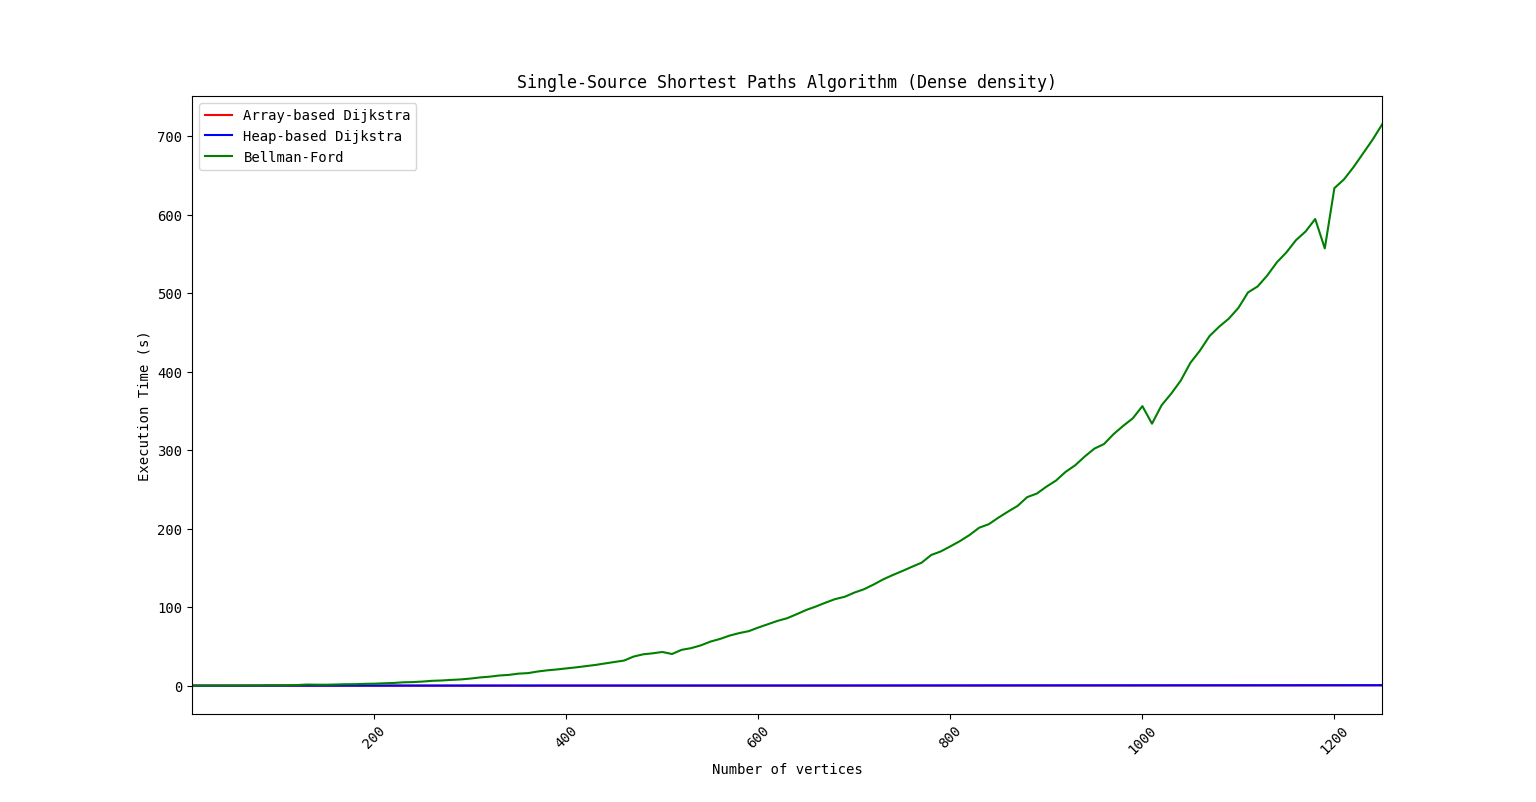
\includegraphics[width=5.5in]{all_dense_01.png}
  \caption{Line charts depicting the performance (\emph{in terms of time} (\(s\))) of the Bellman-Ford, Array-based Dijkstra and Binary-Heap based Dijkstra approaches with respect to dense graphs.}
  \label{fig6:dense1}
\end{figure}

\begin{figure}[H]
  \centering
  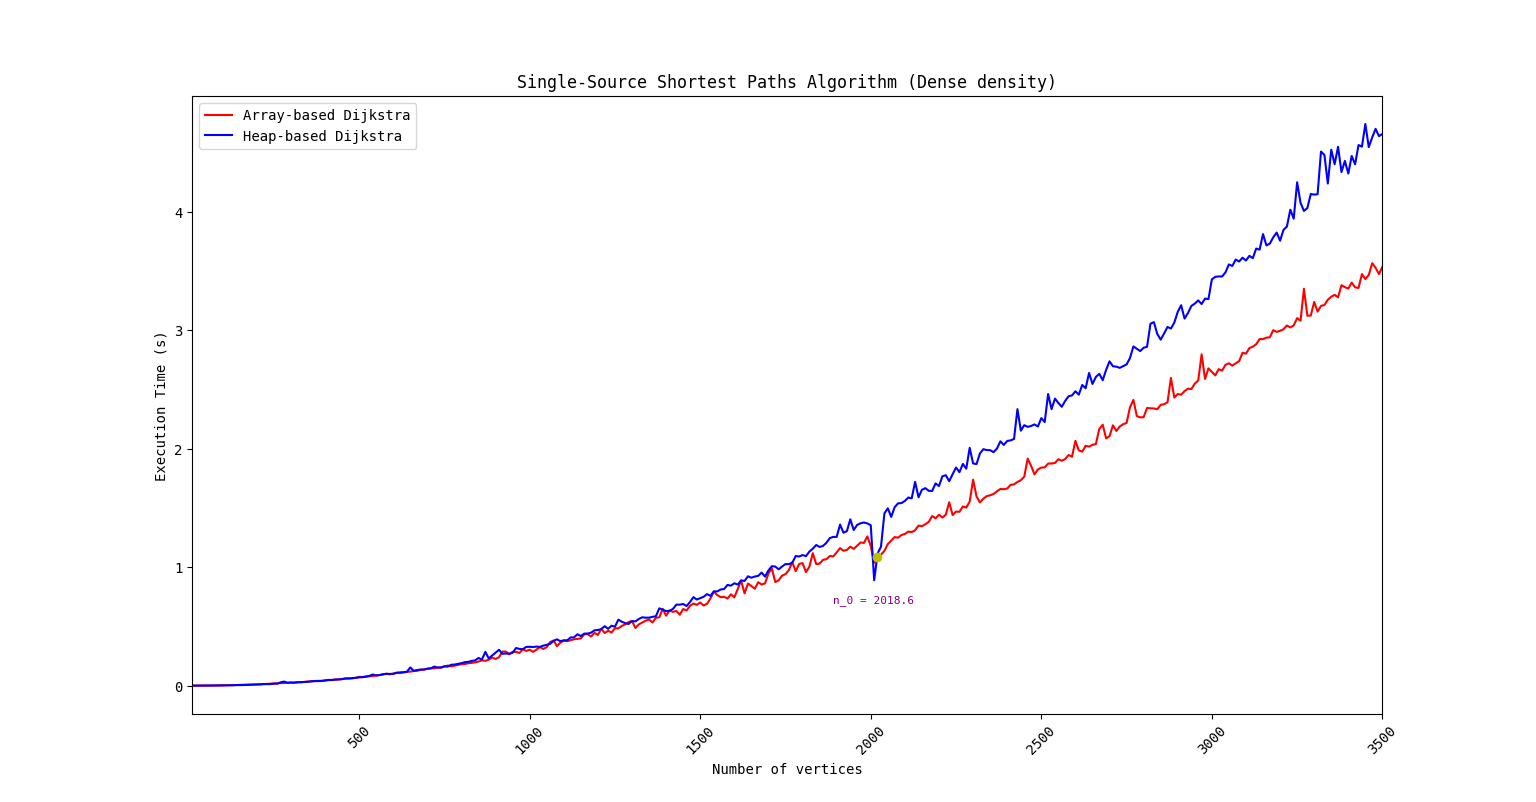
\includegraphics[width=5.5in]{all_dense_02.png}
  \caption{Line charts depicting the performance (\emph{in terms of time} (\(s\))) of the Array-based Dijkstra and Binary-Heap based Dijkstra approaches with respect to dense graphs.}
  \label{fig7:dense2}
\end{figure}

From \textbf{Figures} \ref{fig6:dense1} and \ref{fig7:dense2} a clear heirarchy can be seen in terms of performance. Ranking the algorithms (\emph{fastest to slowest}), we get:
\begin{enumerate}
  \item Array-based Dijkstra
  \item Binary Heap-baed Dijkstra
  \item Bellman-Ford
\end{enumerate}

To understand what was happened here, we must remember what class of input we are dealing with. From \textbf{Section} \ref{sec:5.1.1}, we have that this dense class of graphs has every single possible edge between evey single pair of vertices. Moreover,
we know that these graphs are directed and strongly conencted. Thus, we know for a fact that in this case the total number of edges is \emph{\textbf{exactly}} equal to the maximal number of edges $\implies |V| \cdot (|V| - 1)$ \cite{cormenBk}. Hence, the following relation holds:
\begin{equation}
  \label{eq:relation}
  E = \Theta(|V|^{2})
\end{equation}
Now, Bellman-Ford has a complexity of $O(|V||E|)$. Thus, by (\ref{eq:relation}), we have that Bellman-Ford, \emph{in this particular case}, has a runtime of $\Theta(|V|^{3})$.

By the same token, we can reason for the Binary-Heap implementation of Dijkstra as well. Now, this variant of Dijkstra has a runtime of \(O(|E| \log |V|)\) thus, by (\ref{eq:relation})
we get that this approach has, \emph{in this particular case}, a runtime of $\Theta(|V|^{2} \log |V|)$. 

Finally, with respect to the Array-based implementation of Dijkstra, we have that with this particular class of input, the runtime is: $O(|V|^{2} + |E|) \implies O(|V|^{2} + |V|^{2}) \implies O(2|V|^{2}) \implies O(|V|^{2})$.
This particular algorithm does not suffer, \emph{asymptotically atleast}, a pile-on effect induced by the \(|E|\) factor, all because of two reasons:
\begin{itemize}
  \item By the greedy strategy in play, each edge is effectively examined only once thus, a total of $|E|$ relaxations occur \cite{cormenBk,ocw:2020,stand:bford:12}.
  \item Relaxation is constant time operation \cite{cormenBk,ocw:2020,stand:bford:12}.
\end{itemize}

\subsubsection{Average}

\begin{figure}[H]
  \centering
  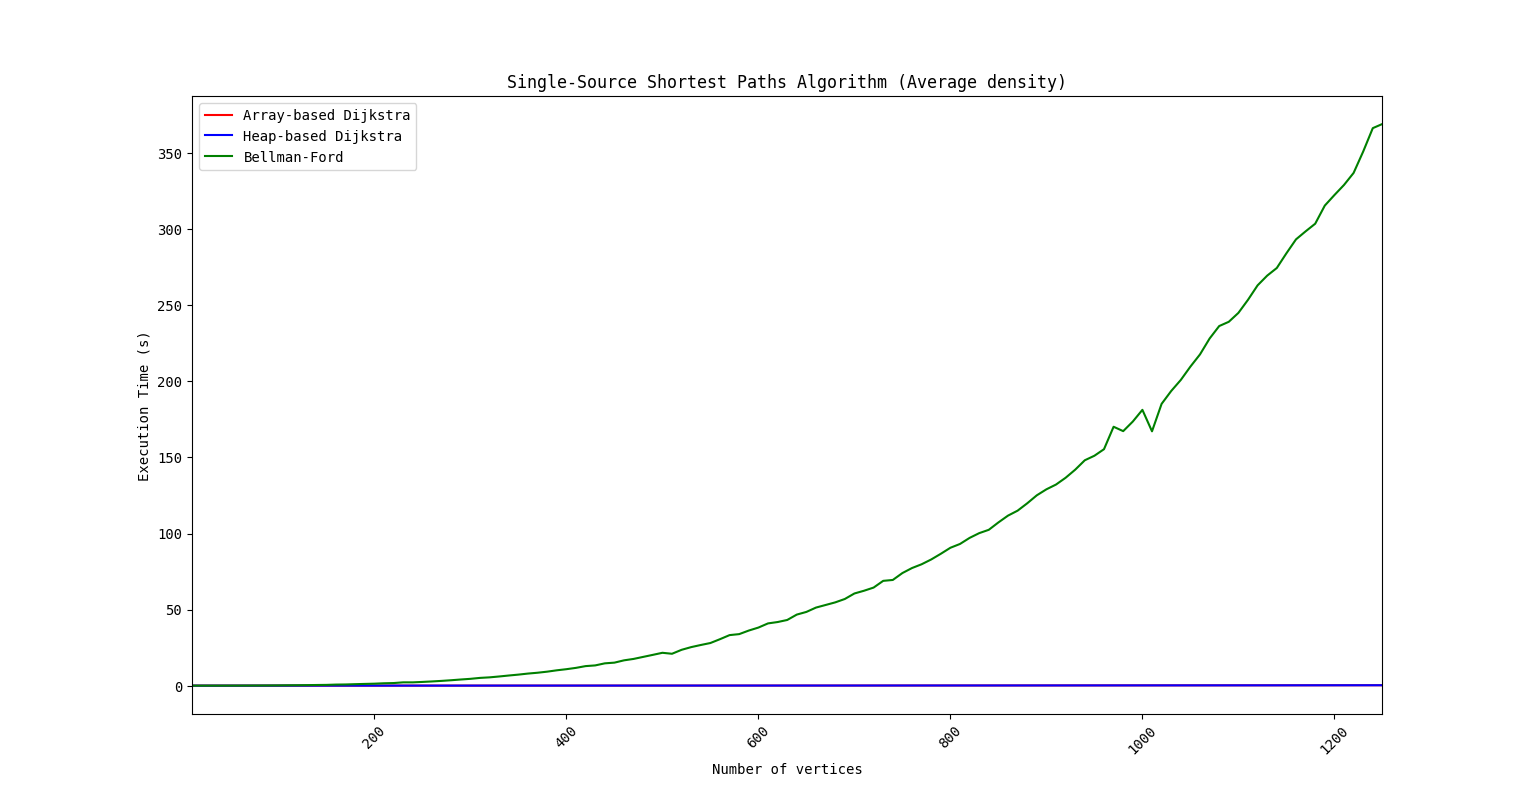
\includegraphics[width=5.5in]{all_average_01.png}
  \caption{Line charts depicting the performance (\emph{in terms of time} (\(s\))) of the Bellman-Ford, Array-based Dijkstra and Binary-Heap based Dijkstra approaches with respect to average density graphs.}
  \label{fig8:avg1}
\end{figure}

\begin{figure}[H]
  \centering
  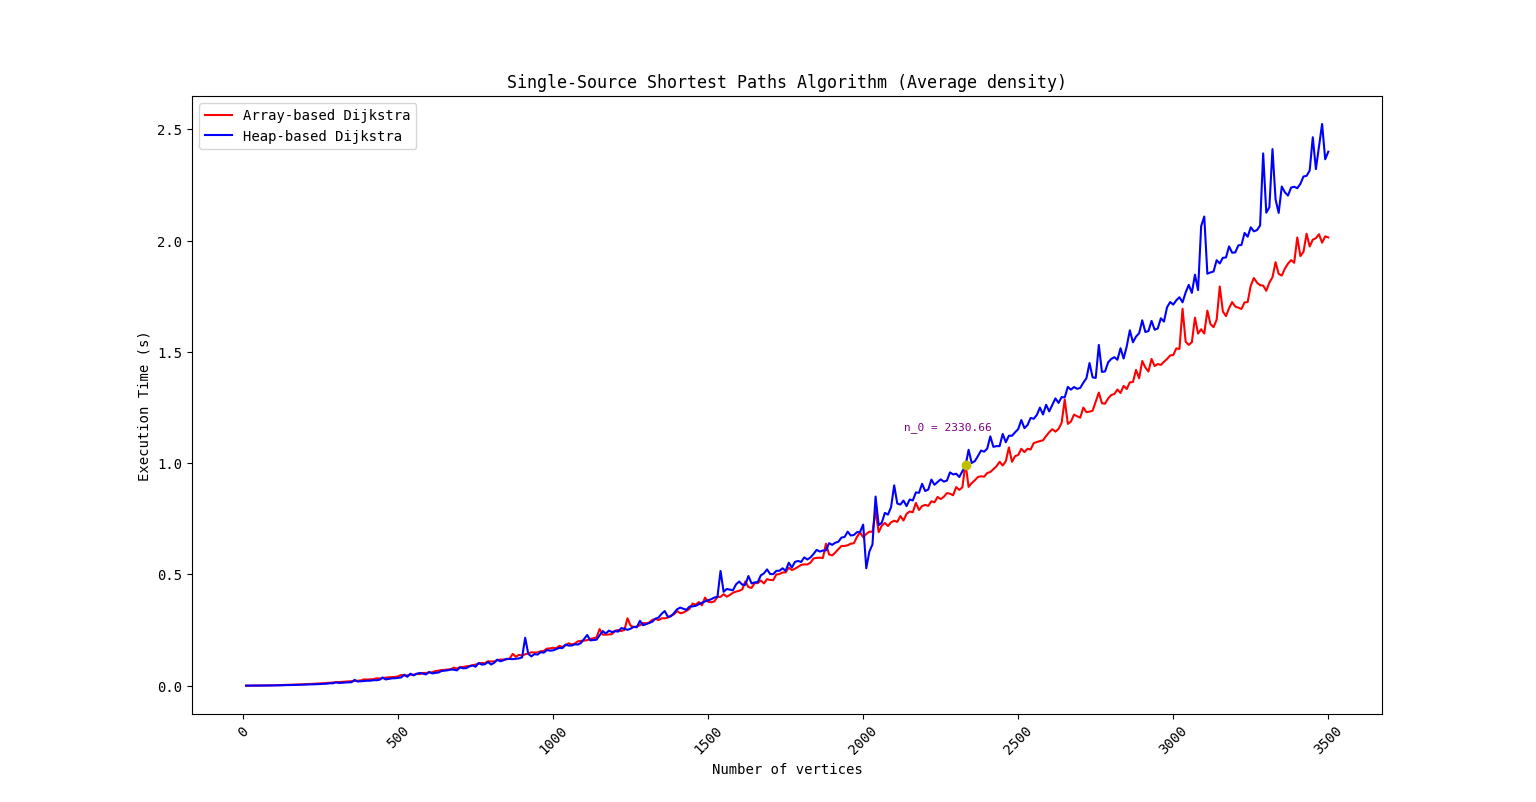
\includegraphics[width=5.5in]{all_average_02.png}
  \caption{Line charts depicting the performance (\emph{in terms of time} (\(s\))) of the Array-based Dijkstra and Binary-Heap based Dijkstra approaches with respect to average density graphs.}
  \label{fig9:avg2}
\end{figure}

From \textbf{Figure} \ref{fig8:avg1} and \ref{fig9:avg2}, we see results no different than in the dense case (\emph{though one must take note of the faster running times}). Even with the parameter, \(p = 0.5\)
the ``\emph{average}'' density graphs prove to be \emph{nearly} just as dense as their \(p=1\) counterpart. Thus, the analyses from the dense case hold here as well, the only real difference being that the bounds are not
as tight in this particular case - the edges are \emph{approximately} equal to the maximal number of edges thus, we get:
\begin{equation}
  \label{eq2:relation}
  E = O(|V|^{2})
\end{equation}

\subsubsection{Sparse}

\begin{figure}[H]
  \centering
  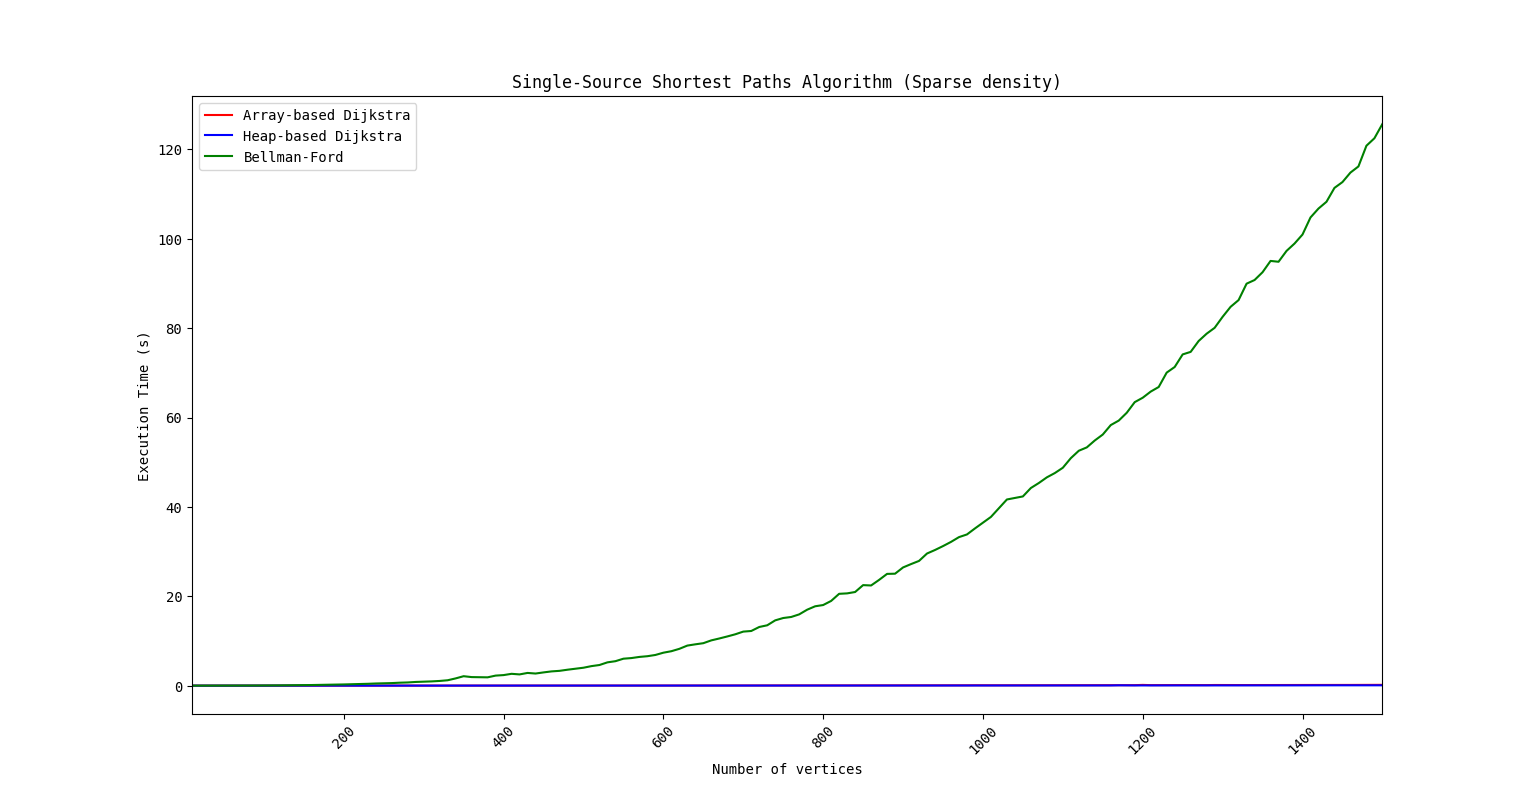
\includegraphics[width=5.5in]{all_sparse_01.png}
  \caption{Line charts depicting the performance (\emph{in terms of time} (\(s\))) of the Bellman-Ford, Array-based Dijkstra and Binary-Heap based Dijkstra approaches with respect to sparse graphs.}
  \label{fig10:sparse1}
\end{figure}

\begin{figure}[H]
  \centering
  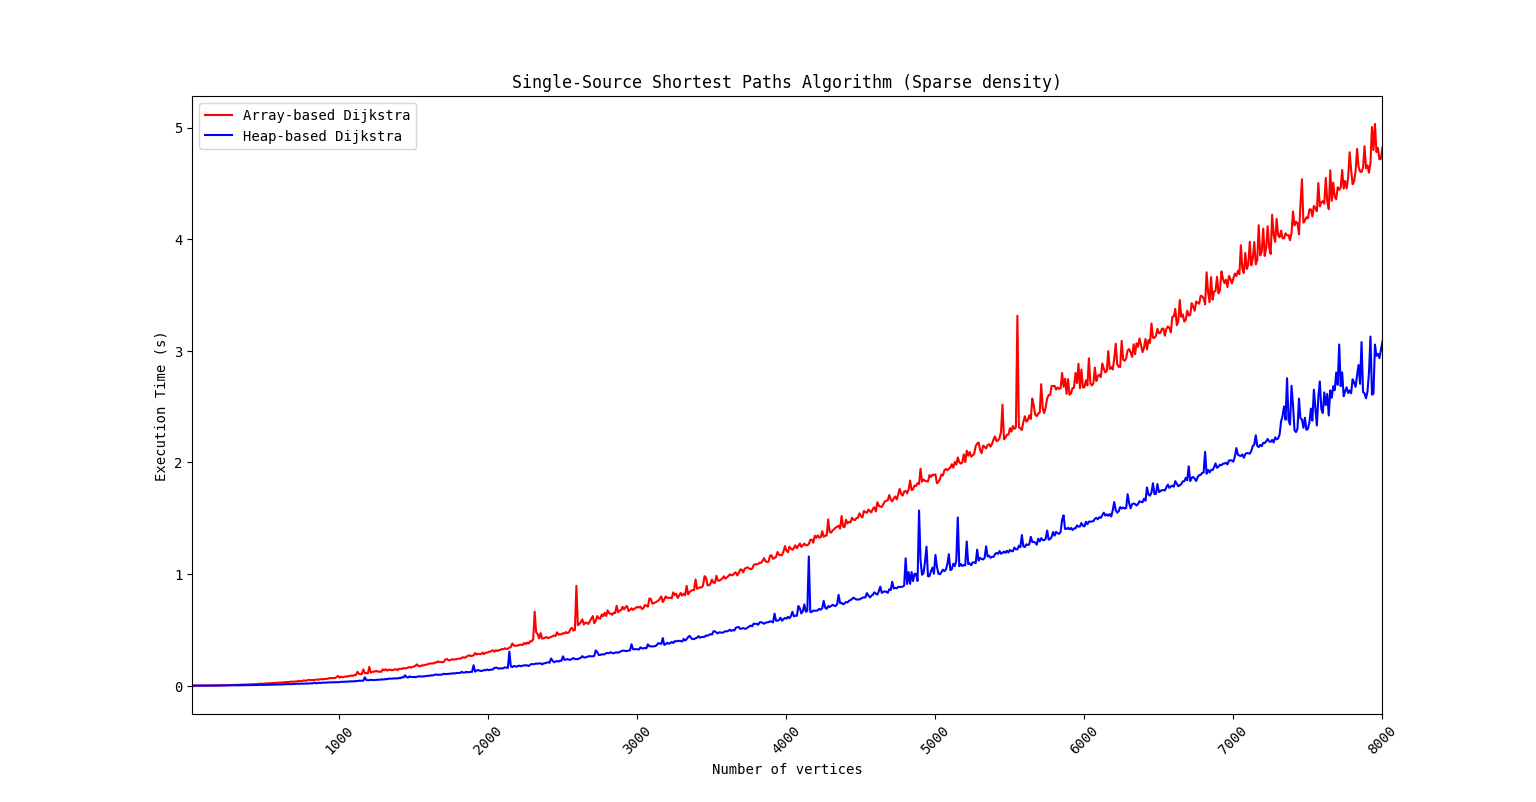
\includegraphics[width=5.5in]{all_sparse_02.png}
  \caption{Line charts depicting the performance (\emph{in terms of time} (\(s\))) of the Array-based Dijkstra and Binary-Heap based Dijkstra approaches with respect to sparse graphs.}
  \label{fig11:sparse2}
\end{figure}

From \textbf{Figures} \ref{fig10:sparse1} and \ref{fig11:sparse2}, it becomes clearly apparent that Bellman-Ford is inherently a slower algorithm than Dijkstra as a whole such that, even with sufficient sparse-ness
the algorithm still persists to be incredibly slow. With respect to the two Dijkstra variants however, things take an incredibly interesting turn. With such a sparse graph, where \(|E|\) is much smaller than the maximal
number of edges \cite{cormenBk}, to be precise:
\begin{equation}
  |E| = o(\frac{|V|^{2}}{\log |V|})
\end{equation}
The complexity for the Array-based Dijkstra gets less optimal becasue of the first term, \(|V|^{2}\). In this case, the Binary-Heap variant improves upon the naive implementation via the array and instead provides
a much faster runtime of, \(O(|E|\log |V|)\) \cite{cormenBk}.  

\chapter{Conclusion}
In conclusion, Dynamic Programming and Greed Algorithms offer wildly different appraoaches to solving the problem of Single-Souce Shortest-Paths. Each of these techniques, through their respective algorithms - Dijkstra and Bellman-Ford
- bring to the shortest path problem their own specific set of intracacies which themselves offer interesting insights both with respect to performance (\emph{the speed by which the problem is solved}) and scope (\emph{how general of an
instance of the problem is solvable}). By comparing the Bellman-Ford and Dijkstra algorithms on both a theoretical and empirical level, one is provided with the answers/insights for both of the aforementioned aspects. By way of comparision
as, has been done here, one may be tempted to resort to a \emph{best-worst} ranking of sorts however, with the correct execution of the execrcise itself, one must realise that such a categorisation is pointless and utterly reductive (\emph{misses the big picture}).
Largely, by the variability in the results seen via the empirical analysis - consider how, specific instances of density leads to a specific variant of Dijkstra being the faster implementation - the
authors have come to realize that there exists a certain scenario (i.e., context) where a particular algorithm/design technique is the most appropriate choice. From the analyses within this project, it is apparent that Bellman-Ford with a 
complexity of \(O(|V|\cdot|E|)\) is the slower algorithm as compared to Dijkstra yet, the very factor that makes it slow is what imbues within it the ability to handle a more general case of input which Dijkstra cannot handle. Additionally,
the Array-based Dijkstra implementation proves to be much faster than its Binary-Heap counterpart yet, it is considerably slow when faced with a sparse graph. Thus, the authors come away with following conclusion:
there is no best/worst algorithm rather, an algorithm that is best suited to specific task or configuration of input. Speaking strictly with respect to the Single-Source Shortest-Paths problem, we conlcude: (i) Bellman-Ford is best suited
to instances, where the graph has negative weights (ii) Array-based Dijkstra is best suited to cases of incredible density of input (iii) Binary-Heap based Dijkstra is best suited to cases of sufficient sparseness.
In short, very rarely is there a \emph{swiss-army knife} situation where one algorithm suits all rather, what we have generally is specific tool for a specific job.

\newpage
\bibliographystyle{acm} % We choose the "acm" reference style
\bibliography{../refs}

\end{document}
